\documentclass{article}
\usepackage[utf8]{inputenc}
\usepackage{minted}
\usepackage{natbib}
\usepackage[spanish]{babel}
\usepackage{graphicx}
\graphicspath{ {imagenes/} }
\usepackage{geometry}
 \geometry{
 a4paper,
 total={170mm,257mm},
 left=35mm,
 right=25mm,
 top=20mm,
 }
\renewcommand{\theenumii}{\theenumi.\arabic{enumii}.}  % 2nd level of enumerate with numbers
\renewcommand{\labelenumii}{\theenumii} % 2ndd level of enumerate with numbers
\author{Adrián Gil Moral }

\newcommand{\cool}[1] {
    {\texttt{#1}}
}

\begin{document}
\section{Solución propuesta}

\paragraph{}
Para el desarrollo de este proyecto se ha utilizado software de terceros que en todas las etapas del mismo ha sido exclusivamente software libre y gratuito motivo por el cual no va a ser señalada esta característica para cada una de las herramientas utilizadas que será citada a continuación. La gratuidad de este software tiene la consecuencia directa de que reduce el precio del desarrollo del proyecto. A su vez, tanto cada uno de los programas que ha sido necesario programar como esta propia memoria están amparados bajo una licencia de Creative Commons para por una parte facilitar la replicación de los experimentos realizados para así cercionarse de la validez del análisis y por otra parte para permitir a terceros desarrolladores obtener el máximo provecho al trabajo desarrollado.

\subsection{Herramientas de desarrollo utilizadas}

\subsubsection{Sistema operativo}

\paragraph{}
El sistema operativo utilizado en cada una de las etapas del proceso ha sido Debian GNU/Linux versión 8.7. Este sistema operativo ha sido elegido para el proyecto ya que por una parte algunos de los programas de terceros desarrolladores están pensados para ser utilizados en sistemas operativos GNU/Linux y por otra se tenía cierta familiaridad previa con el mismo. Este sistema operativo puede descargarse en la siguiente página web: www.debian.org [última vez visitada: 18/05/2017].

\subsection{Edición de código}
\paragraph{}
El código ha sido editado y desarrollado mediante el editor de texto plano Gedit, que es un editor el cual viene incluído en el paquete de instalación básico de muchas distribuciones de GNU-Linux. Puede descargarse en la siguiente página web: www.wiki.gnome.org/Apps/Gedit [última vez visitada: 18/05/2017]. Este editor ha sido utilizado por su sencillez. Sin embargo, para proyectos más complejos puede ser mejor utilizar otros editores como Vim\footnote{www.vim.org} o Emacs\footnote{https://www.gnu.org/software/emacs/}, ambos de software libre y gratuito.

\subsection{Control de versiones}
\paragraph{}
Para el control de versiones de código se ha utilizado un repositorio de Git alojado en una copia remota GitHub con un único repositorio para alojar todo el código utilizado así como otro repositorio para las distintas versiones de la memoria.

\paragraph{}
De esta manera, en caso de pérdida o avería del dispositivo con el que se ha desarrollado este proyecto, existía una copia de seguridad de todo el trabajo realizado en GitHub.

\paragraph{}
Al haberse escrito esta memoria en un formato que antes de ser transformado a PDF es texto plano (en contraposición con el formato de texto enriquecido de editores como LibreOffice Writer), en lugar de usar un repositorio de documentos como Alfresco\footnote{www.alfresco.com}, se ha podido crear otro repositorio de Git que detectase los cambios entre las distintas versiones de la memoria.

\subsection{Edición de la memoria}
\paragraph{}
La memoria ha sido desarrollada en \LaTeX{} (latex) y en este caso por comodidad ha sido escrita en el editor en línea de Sharelatex. Esto es debido únicamente a que a diferencia de lo que ocurre con el editor Gedit estándar (es decir, sin añadir ningún complemento), en este editor en línea es posible comprobar los errores de sintaxis antes de haber compilado el archivo así como el hecho de que la propia interfaz permite visualizar paralelamente el documento PDF que se va a generar y ver la correspondencia entre la salida en dicho PDF con la línea exacta del archivo de latex que la genera. En los anexos se puede encontrar la lista completa de paquetes necesarios para la compilación de esta memoria.

\paragraph{}
Una vez modificados los documentos en Sharelatex, estos eran pasados a Git de forma manual: el proyecto de Sharelatex era descargado y después subido como commit en Git con los cambios que detectase.

\subsection{Scripts para la traducción de problemas manuales}
\paragraph{}
La mayoría de las versiones de los dominios y problemas realizados a mano han sido realizados mediante scripts que tuviesen como parámetro de entrada el problema original y como archivo de salida el problema en la versión modificada a mano correspondiente. Estos scripts se han realizado en el lenguaje de programación Python.

\subsection{Scripts para la generación de problemas automáticos}
\paragraph{}
Los scripts de terceros utilizados para la transformación automática de dominios generan un dominio por cada ejecución. Con el fin de automatizar la transformación de todos los problemas, se han creado varios un script en Bash para cada uno de los modificadores para así poder obtener todos los problemas modificados a partir de aquellos que se encuentren en un directorio especificado sin tener que ejecutar a mano cada uno de estos scripts de transformación por cada uno de los problemas a transformar.

\subsection{Scripts para la automatización de pruebas}
Se ha realizado un script en Bash que permite obtener los tiempos de ejecución y la calidad de la solución de la planificación automática de la versión del dominio y los problemas que se introduzcan como parámetros para los planificadores Metric-FF y LPG. En la sección de evaluación de resultados se concreta exactamente en qué consisten estas pruebas.

\subsection{Descripción de los dominios}

\paragraph{}

En esta sección se van a describir todos los dominios utilizados en el proyecto
como entrada de los distintos planificadores utilizados en la fase de obtención
de tiempos y de calidad de las soluciones para su ulterior análisis. 

\paragraph{}
Todas las versiones de dominios utilizados provienen de la edición de 2014 de la IPC. Mayoritariamente se han realizado modificaciones en el dominio de Childsnack de esta edición. A su vez, se han incluido alguna modificación adicional a otros dominios presentados en esta edición con la única intención de demostrar que este tipo de modificaciones no son algo exclusivo de este dominio sino que la modificación de la representación de un dominio con el fin de mejorar la eficiencia en la búsqueda de la solución es algo extendido que se puede realizar en un gran abanico de dominios, pues es frecuente que la representación de los dominios sea mejorable.

\paragraph{}
Las modificaciones realizadas a dominios que no sean el Childsnack han sido realizadas todas a mano. Por contra, en el dominio de Childsnack se han incluido tanto modificaciones realizadas a mano como modificaciones realizadas mediante software de terceros que es independiente de dominio.

\paragraph{}
En el caso de que uno de los dominios derive de otro, únicamente se va a
explicar en el dominio derivado los motivos y los cambios respecto al dominio
original. Por último, en todos ellos se explicará si los nuevos dominios son
completos y si se pierde la optimalidad respecto al dominio original.

\subsection{Versiones del dominio Childsnack}
\subsubsection{Dominio original}

\paragraph{}
El dominio original recibe el nombre de \textit{ChildSnack} y fue presentado por
primera vez en la edición del año 2014 de la \textit{IPC} (International
Planning Competition). En este dominio se pretende organizar la creación y
distribución de sándwiches a partir de unos componentes con y sin gluten para un
grupo de niños donde parte de ellos puede que sean alérgicos al gluten, por lo
que en este caso los dos componentes de los sándwiches deberán necesariamente no
tener gluten. Por otro lado, en el caso de los niños que no son alérgicos al
gluten será indiferente si alguno o todos los componentes del sándwich contienen
o no gluten.

\paragraph{}
Los sándwiches se definen con el predicado \textit{(at\_kitchen\_sandwich ?s -
sandwich)} y constan de dos componentes: el pan y el contenido, que son
definidos mediante los predicados \textit{(at\_kitchen\_bread ?b - bread-portion)}
y \textit{(at\_kitchen\_content ?c - content-portion)}. Todos los sándwiches se hacen
en la cocina (que se define a su vez mediante la constante \textit{kitchen}) y
únicamente se gasta un trozo de pan y de componente por cada sándwich. En la
definición original del dominio, únicamente se puede definir la cocina como
localización de los componentes del sándwich, a diferencia de lo que ocurre con
los bandejas portátiles, los sándwiches y los niños. Una vez se ha creado el
sándwich, los componentes utilizados son eliminados de la lista de hechos (no
son reutilizables).

\paragraph{}
Como ya se ha comentado, los componentes de los sándwiches así como el sándwich
final podrá tener o no gluten. En caso de que alguno de estos elementos tenga
gluten, no será necesario añadir ningún predicado adicional. Por contra, para
señalar que uno de estos elementos no contiene gluten se utilizará el predicado
correspondiente de los siguientes: \textit{(no\_gluten\_bread ?b - bread-portion)}, \textit{(no\_gluten\_content ?c - content-portion)}, \textit{(no\_gluten\_sandwich
?s - sandwich)}.

\paragraph{}
Los sándwiches que se crean en la cocina pueden después ser cargados y
transportados utilizando bandejas portátiles. Estos bandejas portátiles no tiene
ninguna restricción en cuanto a cantidad de sándwiches que pueden transportar y
permiten que los sándwiches puedan ser transportados libremente entre la cocina
y las distintas localizaciones de los niños, permitiendo a su vez que tanto el
origen como el destino dla bandeja sean distintas posiciones de los niños. Las
bandejas se declaran mediante el predicado \textit{(at ?t - tray ?p - place)}, que
indica la localización de cada una de ellas.

\paragraph{}
En caso de que coincida la localización dla bandeja con la cocina, los
sándwiches que queden creados en la cocina pueden ser cargados en la bandeja
mediante la declaración del predicado \textit{(ontray ?s - sandwich ?t - tray)}. A su
vez, en caso de coincidir la localización dla bandeja con la de alguno de los
niños que aún no haya sido servido y la bandeja esté cargado con algún sándwich
que se adapte a sus necesidades en cuanto al gluten se refiere, este sándwich
puede ser eliminado dla bandeja y servido al niño.

\paragraph{}
Los niños que no han sido servidos y que se espera que tras la resolución del
problema sean servidos son declarados mediante el predicado
\textit{(waiting ?c - child ?p - place)} cuando están esperando y con el
predicado \textit{(served ?c - child)} cuando ya han sido servidos.

\paragraph{}
La dificultad principal de este dominio se basa en la limitación de componentes
sin gluten que son necesarios para la creación de sándwiches para los niños
alérgicos al gluten, ya que en el caso de los no alérgicos cualquier sándwich
servido resolvería el problema. Esto podría implicar por ejemplo que se
utilizase erróneamente un componente sin gluten con otro componente con gluten
que podría ser necesario para crear otro sándwich sin gluten. Sin embargo, en
otra situación podría ocurrir que dicha combinación fuera correcta ya que no
quedase otra opción para servir al niño que queda que no es alérgico al gluten.
A su vez, no se le puede servir a un niño no alérgico al gluten un sándwich
etiquetado como sin gluten, por lo que la solución de hacer tantos sándwiches
sin gluten como permita el dominio y después si hace falta distribuir esos
sándwiches entre los no alérgicos se descarta al no ser una solución válida para
cualquier problema de entrada.

\paragraph{}
Al contrario que ocurre con los componentes, para cada niño es necesario
especificar tanto si son como si no son alérgicos al gluten mediante los predicados \textit{(allergic\_gluten ?c - child)} y \textit{(not\_allergic\_gluten ?c - child)}.

\paragraph{}
A este problema hay que sumarle que ni el número de niños definidos en el
problema ni el número de sándwiches máximos que se pueden realizar, definidos
mediante el predicado \textit{(notexist ?s - sandwich)}, tiene por qué coincidir
con el número y la composición de alérgicos de niños definidos en la meta como
que tienen que ser servidos, por lo que incluso aunque se incluyese conocimiento
del dominio en la resolución del problema por parte del planificador, el
problema seguiría sin ser trivial. De todas maneras, aunque el predicado \textit{(notexist ?s - sandwich)} se puede utilizar para limitar el númer máximo de sándwiches que se pueden realizar, su verdadera función es que exista una correlación de a uno en los sándwiches creados. 


\paragraph{}
Tras haber explicado la idea general del dominio así como sus dificultades a la
hora de resolver los problemas, se va a explicar la entrada y salida de cada una
de las acciones del dominio así como la estructura general que deben tener los
problemas de entrada.

\paragraph{}
Las acciones del dominio original son:
\begin{itemize}
    \item \textbf{make\_sandwich\_no\_gluten}
        \begin{itemize}
            \item \textbf{Precondiciones}: que exista al menos un contenido y un trozo de
            pan donde ambos sean sin gluten y haya al menos un hecho de no
            existencia de sandwich. 
            \item \textbf{Efectos}: eliminación de los dos componentes utilizados y del hecho
            de no existencia de sándwich y creación de un sandwich sin gluten.
        \end{itemize}
    \item \textbf{make\_sandwich}
        \begin{itemize}
            \item \textbf{Precondiciones}: que exista al menos un contenido y un trozo de
            pan con o sin gluten y haya al menos un hecho de no existencia de
            sándwich.
            \item \textbf{Efectos}: eliminación de los componentes utilizados y del hecho de no
            existencia de sándwich y creación de un sandwich etiquetado como
            con gluten (aún en el caso de que ambos elementos utilizados no
            tengan gluten).
        \end{itemize}
    \item \textbf{put\_on\_tray}
        \begin{itemize}
            \item \textbf{Precondiciones}: que exista al menos un sándwich en la cocina y
            que al menos uno de los bandejas portátiles esté en la cocina.
            \item \textbf{Efectos}: carga uno de los sándwiches en uno de los bandejas
            portátiles que esté en la cocina.
        \end{itemize}
    \item \textbf{serve\_sandwich\_no\_gluten}
        \begin{itemize}
            \item \textbf{Precondiciones}: que al menos uno de los bandejas portátiles esté
            en la misma posición que uno de los niños, que la bandeja que cumpla
            la precondición anterior tenga al menos un sándwich sin gluten, que
            un niño no alérgico al gluten esté en la misma localización que la
            bandeja que cumple las precondiciones anteriores y que este mismo niño esté esperando un sándwich.
            \item \textbf{Efectos}: el niño pasa a estar servido y se elimina el sándwich utilizado en la operación.
        \end{itemize}
    \item \textbf{serve\_sandwich}
        \begin{itemize}
            \item \textbf{Precondiciones}: que al menos uno de los bandejas portátiles esté
            en la misma posición que uno de los niños, que la bandeja que cumpla la
            precondición anterior tenga al menos un sándwich con o sin gluten,
            que un niño no alérgico al gluten esté en la misma localización que la
            bandeja que cumple las precondiciones anteriores y que este mismo
            niño esté esperando un sándwich.
            \item \textbf{Efectos}: el niño pasa a estar servido y se elimina el sándwich
            utilizado en la operación.
        \end{itemize}
    \item \textbf{move\_tray}
        \begin{itemize}
            \item \textbf{Precondiciones}: que exista al menos un bandeja.
            \item \textbf{Efectos}: mueve la bandeja de su localización inicial a una nueva
            localización.
        \end{itemize}
    
\end{itemize}

\paragraph{}
En el problema se podrán definir los siguientes elementos:
\begin{itemize}
    \item bandejas portátiles, con la localización inicial de cada uno de ellos.
    \item Panes que se encuentran en la cocina.
    \item Contenidos (de los sándwiches) que se encuentran en la cocina.
    \item Especificación de los trozos de pan que no llevan gluten.
    \item Especificación de los contenidos que no llevan gluten.
    \item Especificación de los niños alérgicos al gluten.
    \item Especificación de los niños que no son alérgicos al gluten.
    \item Especificación de los niños que están esperando que les sirvan un sándwich y su localización.
    \item El número máximo de sándwiches que se pueden hacer.
    \item Especificación de los niños que tienen que ser servidos para resolver el problema.
\end{itemize}


\subsubsection{Dominios modificados a mano}
\subsubsubsection{Dominio 01}

\paragraph{}
Mientras que la definición de los problemas en este dominio no varía
respecto a la definición original, en la definición del dominio se han añadido un
macrooperador de las acciones \textit{move\_tray} con las acciones
\textit{serve\_sandwich} y
\textit{serve\_sandwich\_no\_gluten}, quedando por tanto los macrooperadores \\
\textit{move\_tray\_serve\_sandwich} y \textit{move\_tray\_serve\_sandwich\_no\_gluten}. Estas
modificaciones lo que hacen es unir la acción de mover la bandeja con la acción de
servir el sándwich ya que viendo la resolución de problemas se puede comprobar
con facilidad que la solución óptima tras mover la bandeja a una mesa es servir
al menos un sándwich, ya que el objetivo de dicho desplazamiento es
exclusivamente servir dicho sándwich que además es justo la siguiente acción a realizar,
por lo que intuitivamente tiene sentido unir ambas acciones, así como añadir
una acción para mover la bandeja a la cocina para volver a cargarlo.

\paragraph{}
Los nuevos macrooperadores incrementan el número de parámetros de las
precondiciones del operador, pasando de dos a cuatro. A su vez, implica
aumentar el factor de ramificación, ya que se ha aumentado en dos en uno el número de
operadores disponibles.

\paragraph{}
En lo que concierne tanto a la completitud y a la optimalidad, siempre que se
añadan macro-operadores sin eliminar los operadores originales ambas
condiciones se conservarán, puesto que en el peor de los casos en los que no se pueda
obtener la solución óptima o completa utilizando los macro-operadores, siempre
estará la opción de utilizar los operadores originales. En este caso, si se eliminasen
los operadores originales \textit{move\_tray}, \textit{serve\_sandwich} y \textit{serve\_sandwich\_no\_gluten}
contenido en los nuevos macro-operadores y se añadiese a su vez el operador
\textit{move\_tray\_kitchen}, el dominio sería completa puesto que todas las soluciones
del dominio original están contenidas en el nuevo dominio. Sin embargo, este
dominio no sería óptimo puesto que al perder el operador \textit{move\_tray}, en todos
los problemas en los que los niños estuvieran en varias localizaciones, sería
necesario que una vez servido a el/los niño/s de la primera localización, se volviese
necesariamente a la cocina para poder volver a mover la bandeja y servir a el/los
siguiente/s niño/s, perdiendo por tanto la solución óptima al tener que realizar
el movimiento innecesario respecto al dominio original de tener que volver a la
cocina para poder servir el/los siguiente/s sándwich/es. Para que quede este
punto más claro, se va a mostrar un ejemplo de un problema muy sencillo en
el que se puede ver claramente cómo se produce esta pérdida de la solución
óptima.

\paragraph{}
Definición del problema de ejemplo:
\begin{itemize}
    \item Pan \textit{bread1} con gluten
    \item Pan \textit{bread2} sin gluten
    \item Contenido \textit{content1} con gluten
    \item Contenido \textit{content2} sin gluten
    \item Niño \textit{child1} alérgico al gluten
    \item Niño \textit{child2} no alérgico al gluten
    \item Niño \textit{child1} en table1
    \item Niño \textit{child2} en table1
    \item bandeja \textit{tray1} en kitchen
\end{itemize}

\textbf{Solución óptima con el dominio original}: \\

\noindent 0: (MAKE\_SANDWICH\_NO\_GLUTEN SANDW1 BREAD1 CONTENT1) \\
1: (MAKE\_SANDWICH SANDW2 BREAD2 CONTENT2) \\
2: (MAKE\_SANDWICH SANDW3 BREAD3 CONTENT3) \\
3: (PUT\_ON\_TRAY SANDW1 TRAY1) \\
4: (PUT\_ON\_TRAY SANDW2 TRAY1) \\
5: (PUT\_ON\_TRAY SANDW3 TRAY1) \\
6: (MOVE\_TRAY TRAY1 KITCHEN TABLE1) \\
7: (SERVE\_SANDWICH\_NO\_GLUTEN SANDW1 CHILD1 TRAY1 TABLE1) \\
8: (SERVE\_SANDWICH SANDW2 CHILD2 TRAY1 TABLE1) \\
9: (SERVE\_SANDWICH SANDW3 CHILD3 TRAY1 TABLE1) \\

\paragraph{}
\textbf{Solución con el dominio 01 \underline{sin} los operadores iniciales}: \\
\noindent 0: (MAKE\_SANDWICH SANDW3 BREAD3 CONTENT3) \\
1: (MAKE\_SANDWICH SANDW2 BREAD2 CONTENT2) \\
2: (MAKE\_SANDWICH SANDW1 BREAD1 CONTENT1) \\
3: (PUT\_ON\_TRAY SANDW1 TRAY1) \\
4: (PUT\_ON\_TRAY SANDW2 TRAY1) \\
5: (PUT\_ON\_TRAY SANDW3 TRAY1) \\
6: (MOVE\_TRAY\_SERVE\_SANDWICH\_NO\_GLUTEN TRAY1 KITCHEN TABLE1 SANDW1 CHILD1) \\
7: (MOVE\_TRAY\_KITCHEN TRAY1 TABLE1) \\
8: (MOVE\_TRAY\_SERVE\_SANDWICH TRAY1 KITCHEN TABLE1 SANDW2 CHILD2) \\
9: (MOVE\_TRAY\_KITCHEN TRAY1 TABLE1) \\
10: (MOVE\_TRAY\_SERVE\_SANDWICH TRAY1 KITCHEN TABLE1 SANDW3 CHILD3) \\

\paragraph{}
\textbf{Solución con el dominio 01 \underline{con} los operadores iniciales}: \\
\noindent 0: (MAKE\_SANDWICH\_NO\_GLUTEN SANDW1 BREAD1 CONTENT1) \\
1: (MAKE\_SANDWICH SANDW2 BREAD2 CONTENT2) \\
2: (MAKE\_SANDWICH SANDW3 BREAD3 CONTENT3) \\
3: (PUT\_ON\_TRAY SANDW1 TRAY1) \\
4: (PUT\_ON\_TRAY SANDW2 TRAY1) \\
5: (PUT\_ON\_TRAY SANDW3 TRAY1) \\
6: (MOVE\_TRAY\_SERVE\_SANDWICH\_NO\_GLUTEN TRAY1 KITCHEN TABLE1 SANDW1 CHILD1) \\
7: (SERVE\_SANDWICH SANDW2 CHILD2 TRAY1 TABLE1) \\
8: (SERVE\_SANDWICH SANDW3 CHILD3 TRAY1 TABLE1) \\

\paragraph{}
Como se puede ver, estando la bandeja ya en la misma posición que \textit{child2} y \textit{child3}, sin los operadores iniciales necesita volver a la cocina para poder servirles, por lo que queda demostrado con este ejemplo que los operadores son necesarios para conservar la optimalidad. Por este motivo, se van a conservar dichos operadores en la versión final de \textit{domain-01}.

\subsubsection{Dominio 02}

\paragraph{}
La defición de los problemas no varía respecto a la definición original, por lo que en las siguientes líneas se va a explicar en qué varía este nuevo dominio respecto a la definición original. Únicamente se han modificado las precondiciones de único operador \textit{make\_sandwich}. En el dominio original, todos los sándwiches creados con este operador son etiquetados como que tuvieran gluten aún cuando ambos componentes utilizados no contengan gluten. Este supuesto no tiene ningún sentido, ya que implica que se están etiquetando erróneamente sándwiches que realmente no tienen gluten por haber pasado por este operador en lugar de por el operador \textit{make\_sandwich\_no\_gluten}, lo que implica que el propio operador permite que se generen ramas del árbol de decisión que bien son erróneas, bien podrían producirse a través del otro operador mencionado, por lo que están duplicados. Únicamente tendría razón de ser este operador si entre las precondiciones de \textit{serve\_sandwich} se encontrase que los niños no alérgicos al gluten no pueden consumir sándwiches sin gluten, pero no es el caso.

\paragraph{}
Para entender mejor esta modificación, se va a incluir un problema base con un posible árbol de decisión con el dominio original y otro árbol de decisión con este nuevo dominio.

\paragraph{}
El problema en cuestión es el siguiente:
\begin{itemize}
    \item 1 pan sin gluten
    \item 1 componente sin gluten
    \item 1 bandeja en la cocina
    \item 1 niño alérgico al gluten en table1
\end{itemize}

\begin{figure}[H]
    \centering
    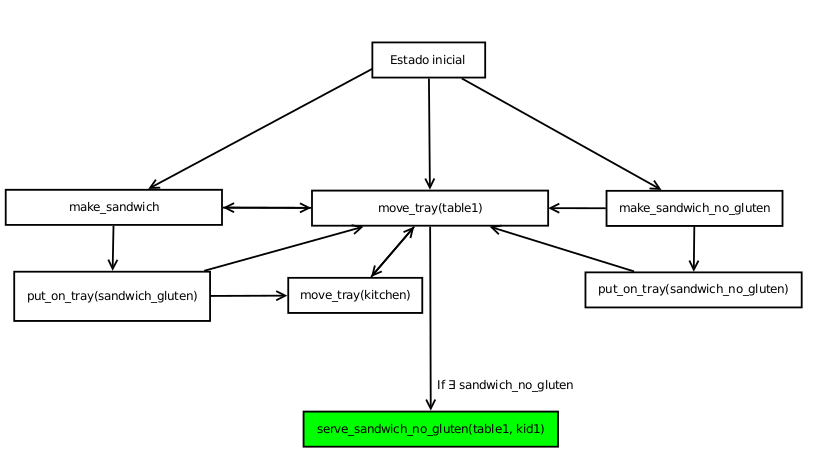
\includegraphics[width=\textwidth, height=8cm]{domain-02-1}
    \caption{Árbol de decisión con el dominio original}
\end{figure}

\begin{figure}[H]
    \centering
    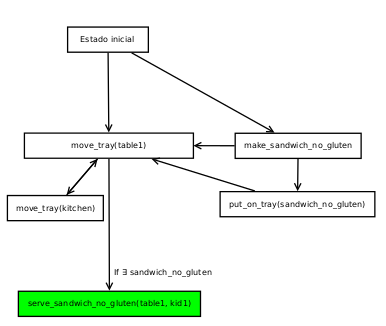
\includegraphics[width=\textwidth, height=8cm]{domain-02-2}
    \caption{Árbol de decisión con el dominio-02}
\end{figure}


\paragraph{}
Como se puede ver, el árbol de decisión del dominio 02 es un subconjunto del árbol de decisión del dominio original. Dicho de manera más genérica, este nuevo dominio sirve para podar el árbol de decisión original para el subconjunto de los problemas posibles en los que existen niños alérgicos al gluten y que por tanto con en el dominio original el planificador podría perder tiempo buscando en ramas del árbol de decisión que se sabe a priori que no van a conducir a la solución.

\paragraph{}
Esto quiere decir que este nuevo dominio es completo y óptimo, pues lo único que se ha hecho ha sido una poda de una rama del árbol de decisión que sólo conduce a soluciones erróneas.

\subsubsection{Dominio 03}

\paragraph{}
Esta versión mantiene la definición de los problemas original, variando exclusivamente la definición del dominio. Esta versión, al igual que la versión 01 se basa en la utilización de macro-operadores, pero llevando su uso hasta el extremo. En este dominio, se han implementado los macro-operadores \\ \textit{ make\_sandwich\_move\_tray\_serve\_sandwich\_move\_tray\_kitchen}, \\ \textit{make\_sandwich\_move\_tray\_serve\_sandwich\_no\_gluten\_move\_tray\_kitchen} y \\ \textit{move\_tray} que sustituirían a todos los demás operadores. Estos dos primeros operadores tendrían como precondiciones que existiese al menos un componente y un trozo de pan con o sin gluten (según cuál de los dos operadores sea), que haya una bandeja en la cocina y que exista un niño alérgico o no al gluten (igualmente, según el operador que corresponda) esperando a ser servido. En caso de que se dé este supuesto, estos operadores producirían un sándwich, lo cargarían en una bandeja, lo transportarían hasta donde está el niño, servirían al niño y traerían la bandeja de vuelta a la cocina.

\paragraph{}
Este macro-operador reduce el árbol de decisión en tanto que existen únicamente tres operadores que se pueden utilizar. Sin embargo, el árbol de decisión contiene un estado por cada instancia posible del operador, valor directamente proporcional al número de parámetros de entrada de dicho operador, que en este caso es muy elevado. La relación entre la pérdida de estados del árbol de decisión debido a la disminución de operadores encapsulados en nuevos macro-operadores y la ganancia de estados en el árbol de decisión debido al incremento de instancias del nuevo operador se llama utilidad y será analizada en la sección de resultados de ejecución.

\paragraph{}
Si no se incluyesen los operadores originales, esta versión sería completa pero no óptima, puesto que no se podría servir a más de un niño sin tener que pasar por la cocina. Por tanto, en esta versión se conservan los operadores originales para no perder la optimalidad.

\subsubsection{Dominio 05}

\paragraph{}
En esta versión, varía tanto la definición del problema como la definición del dominio. Se trata de un dominio numérico con palabras, en las que se definen de manera numérica el número de panes, contenidos, sándwiches con y sin gluten. Los niños no son definidos de manera numérica ya que en la definición original en la meta se especifica los niños concretos (con su respectiva localización) que deben ser servidos, por lo que si fuesen definidos de manera numérica los niños servidos con un operador como \textit{served\_childs ?num - num} se perdería esta capacidad para especificar no sólo el número sino los niños concretos dentro de todos los definidos en el problema que deben ser servidos para la correcta resolución del problema.

\paragraph{}
Los nuevos predicados utilizados son \\ \textit{(at\_kitchen\_bread ?gluten - num ?no-gluten - num)},  \textit{(at\_kitchen\_content ?gluten - num ?no-gluten - num)}, \textit{(at\_kitchen\_sandwich ?gluten - num ?no-gluten - num)} y \textit{(ontray ?gluten - num ?no-gluten - num ?t - tray)} que definen respectivamente el número de panes, contenidos y sándwiches en la cocina y los sándwiches que se encuentran en las bandejas que tengan o no gluten. A su vez, se ha añadido el predicado \textit{(next ?minor - num ?major - num)} que sirve para incrementar y decrementar en una unidad los valores numéricos de los predicados definidos anteriormente. Los predicados del dominio original \textit{(allergic\_gluten ?c - child)}, \textit{(not\_allergic\_gluten ?c - child)}, \textit{(waiting ?c - child ?p - place)}, \textit{(at ?t - tray ?p - place)} y \textit{(served ?c - child)} se han mantenido.

\paragraph{}
Aunque la apariencia es totalmente distinta, la lógica de los operadores es la misma que en el caso original pero adaptada a estas nuevas definiciones numéricas con palabras. Únicamente ha sido necesario incluir el operador \textit{make\_sandwich\_bread\_no\_gluten} y \textit{make\_sandwich\_content\_no\_gluten} que crea \\ sándwiches con gluten con el pan o el contenido sin gluten.

\paragraph{}
Los operadores numéricos comprueban la existencia de lo que serían los \\ parámetros necesarios en el dominio original no a través de la comprobación de la existencia de por ejemplo el nuevo parámetro \textit{(at\_kitchen\_bread ?gluten - num ?no-gluten - num)}, pues siempre va a existir, sino de los valores numéricos contenidos en estos parámetros que en este caso determinan cuántos panes con y sin gluten existen en la cocina. Es decir, en la definición del nuevo problema se definen la lista de sucesión de valores numéricos mediante parámetros como \textit{(next number\_0 number\_1)} o \textit{(next number\_1 number\_2)}, lo que permite tanto sumar y restar una unidad como saber cuál es el menor valor posible que se puede definir (en este caso, el cero). Así, la comprobación que habría que hacer en este dominio para poder decrementar o incrementar un valor de un parámetro es si existe dicho sucesor o predecesor de dicho valor entre las definiciones del problema. Si no tienes predecesor de un número por ejemplo, sabes que el valor que tiene es cero.

\paragraph{}
Para que esto se entienda mejor se van a explicar el funcionamiento de uno de los operadores, por ejemplo de \textit{make\_sandwich\_no\_gluten}. Las precondiciones que tiene este operador son que existan los parámetros \textit{(at\_kitchen\_bread ?bread-gluten ?bread-no-gluten)}, \\ \textit{(at\_kitchen\_content ?content-gluten ?content-no-gluten)} y \textit{(at\_kitchen\_sandwich ?sandwich-gluten ?sandwich-no-gluten)}, que exista el predecesor del pan y el contenido para saber que existe al menos una unidad de cada uno de los componentes que se van a utilizar (\textit{(next ?bread-no-gluten-minor ?bread-no-gluten)} y \textit{(next ?content-no-gluten-minor ?content-no-gluten)}) y que exista el sucesor del sándwich que se va a generar para que se pueda incrementar el número de sándwiches (\textit{(next ?sandwich-no-gluten ?sandwich-no-gluten-major)}). El número máximo de sándwiches por tanto está definido por el mayor número definido en un parámetro \textit{(next ?n ?maximo)}, siendo el valor de \textit{?maximo} el número de cláusulas \textit{notexist} del problema original. Finalmente, este operador elimina los parámetros iniciales (\textit{(not (at\_kitchen\_bread ?bread-gluten ?bread-no-gluten))}, \textit{(not (at\_kitchen\_content ?content-gluten ?content-no-gluten))} y \textit{(not (at\_kitchen\_sandwich ?sandwich-gluten ?sandwich-no-gluten)}) para poder incrementar o decrementar sus valores (\textit{(at\_kitchen\_bread ?bread-gluten ?bread-no-gluten-minor)}, \textit{(at\_kitchen\_content ?content-gluten ?content-no-gluten-minor)} y \textit{(at\_kitchen\_sandwich ?sandwich-gluten ?sandwich-no-gluten-major)}).

\paragraph{}
Por último, esta solución es completa y óptima, puesto que es una redefinición de los operadores originales para adaptarlos a la lógica de un dominio numérico con palabras que sin embargo conserva por completo la lógica inicial del problema, por lo que a diferencia de otras versiones como en la 01 que es necesario conservar los operadores originales para no perder la optimalidad, en este caso no es necesario, pues todas las acciones del dominio original se pueden realizar de manera atómica en este dominio (a diferencia de lo que ocurre con los dominios que usan macro-operadores, que es necesario realizar varias acciones de las acciones agrupadas en el nuevo dominio para la realización de acciones individuales del dominio original). A continuación se incluye la definición de uno de los problemas.

\subsubsection{Dominio 09}

\paragraph{}
En esta versión se modifican tanto los problemas como el dominio. La modificación realizada consiste en eliminar el parámetro \textit{(waiting ?c - child ?p - place)} para incluir la posición de los niños en \textit{(allergic\_gluten ?c - child ?p - place)} y \textit{(not\_allergic\_gluten ?c - child ?p - place)}. La idea de esta modificación es que los parámetros \textit{waiting} y \textit{allergic\_gluten} o \textit{not\_allergic\_gluten} siempre aparecen juntos en los mismos operadores para referirse al mismo valor de \textit{child}, por lo que con esta modificación se intenta comprobar si este tipo de uniones de parámetros que coincide su uso en los mismos operadores reduce o no el tiempo de búsqueda.

\paragraph{}
Los únicos operadores que ha sido necesario modificar son \textit{serve\_sandwich} y \textit{serve\_sandwich\_no\_gluten}, cambiando simplemente los parámetros de \textit{(waiting ?c ?p)} y de bien \textit{(allergic\_gluten ?c)} o \textit{(not\_allergic\_gluten ?c)} por los nuevos parámetros \textit{(allergic\_gluten ?c - child ?p - place)} y \textit{(not\_allergic\_gluten ?c - child ?p - place)}. A continuación se incluye un problema definido para esta versión.

\paragraph{}
Esta versión es completa y óptima puesto que sólo se ha cambiado la representación de los parámetros de algunos operadores pero no se ha modificado la funcionalidad original de los mismos.

\subsubsection{Dominio 11}

\paragraph{}
Esta versión requiere de la modificación de tanto los dominios como de los problemas, y la modificación consiste en eliminar el parámetro \textit{(not\_allergic\_gluten ?c - child)} para tratarlo en los operadores como la negación del parámetro \textit{(allergic\_gluten ?c - child)}, es decir, como \textit{(not(allergic\_gluten ?c - child))}. Esto implica eliminar en los problemas los parámetros \textit{(allergic\_gluten ?c - child)} y modificar únicamente el operador \textit{serve\_sandwich} para definir al niño no alérgico al gluten que se le va a servir el sándwich de la manera que se ha decrito en la oración anterior. Un ejemplo de problema definido de esta forma sería el siguiente.

\paragraph{}
Esta versión es completa y óptima, puesto que es un cambio en la representación de la lógica, pero permanece la lógica de la versión original.

\subsubsection{Dominio 12}

\paragraph{}
Esta es con diferencia la versión con mayor conocimiento del dominio. Para la creación de este dominio se ha buscado el método resolutivo que permite obtener siempre la solución óptima para cualquier tipo de problema de entrada para después crear una versión de los dominios y problemas que se acercase lo máximo posible a esta solución. A continuación se  encuentra el algoritmo de resolución óptimo para cualquier tipo de problema.

\begin{enumerate}
    \item Contar el número de niños a los que hay que servir que son alérgicos al gluten y guardar ese valor en \textit{a}.
    \item Contar el número de niños a los que hay que servir que no son alérgicos al gluten y guardar ese valor en \textit{b}.
    \item Hacer \textit{a} sándwiches sin gluten.
    \item Hacer \textit{b} sándwiches con o sin gluten.
    \item Si no existe ninguna bandeja en la cocina, mover una bandeja a la cocina \textit{c}.
    \item Mover (\textit{a} + \textit{b}) sándwiches a la misma bandeja \textit{c}.
    \item Para cada localización \textit{d} en la que exista al menos un niño que tiene que ser servido:
    \begin{enumerate}
        \item Mover la bandeja \textit{c} a \textit{d}.
        \item Para cada niño \textit{e} que se encuentre en \textit{d} y no haya sido servido:
        \begin{enumerate}
            \item Servir el sándwich correspondiente (según sea o no alérgico al gluten) al niño \textit{e} en \textit{d} de la bandeja \textit{c}. 
        \end{enumerate}
    \end{enumerate}
\end{enumerate}

\paragraph{}
En esta versión se ha conseguido replicar este algoritmo realizando las modificaciones en el dominio original que se expresan a continuación.

\paragraph{}
En cuanto a los \textbf{predicados}, el único predicado que se ha suprimido es \textit{(notexist ?s - sandwich)}, ya que su función es limitar el número de sándwiches que se pueden producir y este concepto ya está incluído en los nuevos predicados \textit{(num\_sandwich\_no\_gluten ?n - num)} y \textit{(num\_sandwich\_gluten ?n - num)}. Estos dos predicados son parámetros introducidos por el usuario con el número de sándwiches (definidos en numérico con palabras) con y sin gluten que es necesario hacer y que debe coincidir con el número de niños alérgicos o no al gluten que deben ser servidos. Ambos parámetros no sólo limitan el número de sándwiches que se pueden hacer, ya que en los operadores de creación de sándwiches se verifica que el número de sándwiches restante de cada tipo sea mayor que cero, sino que también limitan los sándwiches con gluten que se pueden hacer y permiten separar los operadores en varias fases, impidiendo por ejemplo que se mueva una bandeja si antes no se han creado todos los sándwiches con y sin gluten que son necesarios. A su vez, se han incluido los predicados \textit{(next ?minor - num ?major - num)}, que sirve para la creación de variables numéricas con palabras tal y como se especifica en el dominio 05, \textit{(not\_trays\_kitchen)} es simplemente un operador creado para suplir la ausencia de comparaciones de tipo \textit{forall} en \textit{PDDL}, que permitiría saber si existen bandejas en la cocina y que en caso de que la posición inicial de ninguna de las bandejas coincida con la cocina, será necesario añadir este predicado en el problema para indicar al dominio que es necesario ejecutar el operador \textit{move\_tray\_kitchen}. El predicado \textit{(first\_load)} se incluye siempre en la definición del problema y sirve para poder saber cuándo se ha realizado la primera carga ya que así a partir de la segunda carga se va a exigir que la bandeja en la que se cargue el sándwich ya contenga al menos un sándwich (consiguiendo con ello que todos los sándwiches se carguen en la misma bandeja, ya que el operador para la primera carga \textit{put\_on\_tray\_first\_load} que permite cargar el sándwich en cualquier bandeja sólo se va a poder ejecutar una única vez). Finalmente, el predicado \textit{(num\_sandwich\_ontray ?n - num)} es inicializado con el número de sándwiches totales con y sin gluten que tienen que realizarse para así poder disminuir en una unidad cada sándwich cargado en la bandeja para que así se pueda poner como limitador de movimiento de las bandejas que ninguna se puede mover hasta que estén cargados todos los sándwiches.

\paragraph{}
Como en esta versión se han realizado importantes modificaciones en los \textbf{operadores}, por lo que van a ser explicados uno a uno como se realizó en el dominio original.

\begin{itemize}
    \item \textbf{make\_sandwich\_no\_gluten}
        \begin{itemize}
            \item \textbf{Precondiciones}: que exista al menos un contenido y un trozo de pan donde ambos sean sin gluten y exista un predecesor del número de sándwich sin gluten por hacer.
            \item \textbf{Efectos}: eliminación de los dos componentes utilizados, decremento del número de sándwiches sin gluten que quedan por hacer y creación de un sandwich sin gluten.
        \end{itemize}
    \item \textbf{make\_sandwich}
        \begin{itemize}
            \item \textbf{Precondiciones}: que exista al menos un contenido y un trozo de pan donde cualquiera o ambos de ellos pueden contener o no gluten, que exista un predecesor del número de sándwich con gluten por hacer y que se hayan hecho todos los sándwiches necesarios sin gluten.
            \item \textbf{Efectos}: eliminación de los dos componentes utilizados, decremento del número de sándwiches con gluten que quedan por hacer y creación de un sandwich etiquetado como con gluten.
        \end{itemize}
    \item \textbf{move\_tray\_kitchen}
        \begin{itemize}
            \item \textbf{Precondiciones}: que exista el hecho que indica que no hay ninguna bandeja en la cocina y se hayan hecho todos los sándwiches con y sin gluten que había que hacer.
            \item \textbf{Efectos}: mueve una bandeja a la cocina y eliminación del hecho que indica que no hay ninguna bandeja en la cocina para que así no se pueda repetir esta acción con más bandejas y así se pierda la optimalidad.
        \end{itemize}
    \item \textbf{put\_on\_tray\_first\_load}
        \begin{itemize}
            \item \textbf{Precondiciones}: que se hayan hecho todos los sándwiches con y sin gluten que había que hacer, que haya al menos una bandeja en la cocina y que sea la primera carga en una bandeja.
            \item \textbf{Efectos}: carga en una bandeja un sándwich.            
        \end{itemize}
    \item \textbf{put\_on\_tray}
        \begin{itemize}
            \item \textbf{Precondiciones}: que se hayan hecho todos los sándwiches con y sin gluten que había que hacer, que haya al menos una bandeja en la cocina y que la bandeja sobre la que se va a cargar tenga ya al menos un sándwich.
            \item \textbf{Efectos}: carga un sándwich en una bandeja previamente cargada.
        \end{itemize}        
    \item \textbf{move\_tray}
        \begin{itemize}
            \item \textbf{Precondiciones}: que se hayan hecho todos los sándwiches que había que hacer con y sin gluten, que se hayan cargado todos los sándwiches en la bandeja y que en la posición actual no quede ningún niño al que se le pueda servir un sándwich con gluten.
            \item \textbf{Efectos}: mueve la bandeja a una nueva posición.
        \end{itemize}                
    \item \textbf{move\_tray\_no\_gluten}
        \begin{itemize}
            \item \textbf{Precondiciones}: que se hayan hecho todos los sándwiches que había que hacer con y sin gluten, que se hayan cargado todos los sándwiches en la bandeja y que en la posición actual no quede ningún niño al que se le pueda servir un sándwich sin gluten.
            \item \textbf{Efectos}: mueve la bandeja a una nueva posición.
        \end{itemize}                
    \item \textbf{serve\_sandwich\_no\_gluten}
        \begin{itemize}
            \item \textbf{Precondiciones}: que al menos uno de los bandejas portátiles esté en la misma posición que uno de los niños, que la bandeja que cumpla la precondición anterior tenga al menos un sándwich sin gluten, que un niño no alérgico al gluten esté en la misma localización que la bandeja que cumple las precondiciones anteriores y que este mismo niño esté esperando un sándwich.
            \item \textbf{Efectos}: el niño pasa a estar servido y se elimina el sándwich utilizado en la operación.
        \end{itemize}
    \item \textbf{serve\_sandwich}
        \begin{itemize}
            \item \textbf{Precondiciones}: que al menos uno de los bandejas portátiles esté en la misma posición que uno de los niños, que la bandeja que cumpla la precondición anterior tenga al menos un sándwich con o sin gluten, que un niño no alérgico al gluten esté en la misma localización que la bandeja que cumple las precondiciones anteriores y que este mismo niño esté esperando un sándwich.
            \item \textbf{Efectos}: el niño pasa a estar servido y se elimina el sándwich utilizado en la operación.
        \end{itemize}
\end{itemize}

\subsubsection{Planificadores utilizados}
\paragraph{}
Los planificadores utilizados para las pruebas realizadas son Metric-FF en su versión 2.1 y LPG en su versión \textit{td}, teniendo Metric-FF como parámetro de ejecución la opción estándar \textit{-s 0} (en caso de fallar la búsqueda con EHC, iniciar la búsqueda con BFS). Inicialmente también se incluyó el planificador FastDownward utilizando Lama2011 como heurística, pero se descartó este planificador al no ser capaz de resolver ni un solo problema en varias de las versiones. El funcionamiento interno de estos tres planificadores queda expuesto en la sección del estado del arte.

\subsubsection{Métricas utilizadas}
\paragraph{}
Los problemas han sido ejecutados por cada planificador con un tiempo máximo de 30 minutos por cada problema. En caso de no encontrar una solución en ese lapso de tiempo, el problema contabiliza como no resuelto.

\paragraph{}
Las métricas utilizadas para la comparación de los resultados han sido estas tres:
\begin{itemize}
    \item Tiempo necesario para encontrar la solución.
    \item Longitud del plan (en caso de encontrar solución).
    \item Calidad relativa de la solución según la métrica de la IPC. \comment{Add formula and explain it}
\end{itemize}

\subsection{Dominios generados automáticamente}
\paragraph{}
En esta sección se explicará brevemente la composición de los dominios generados automáticamente mediante software independiente de dominio de terceros. Para todos estos dominios se ha utilizado exclusivamente como entrada de los problemas el problema y el dominio original.

\paragraph{}
Como la lógica de estas modificaciones es de otros propietarios, las explicaciones serán bastante menos detalladas que las que aparecen en la sección de los dominios modificados a mano.

\subsubsection{Dominio original-ptt}
\paragraph{}
Este modificador debería transformar el dominio mediante la inclusión de macrooperadores, que como se ha mostrado en la sección de dominios hechos a mano, existen varias alternativas para dicha implementación. Sin embargo, el software de PTT ha sido incapaz de encontrar un solo macrooperador, por lo que tanto la definición del dominio como los problemas generados son los mismos que los introducidos como entrada, por lo que en lo referente a la comparación de los tiempos obtenidos con las distintas versiones esta versión de los problemas va a ser descartada, al ser exactamente igual que la versión original del problema.\footnote{En ejecuciones de este software con otras versiones de este dominio, se ha comprobado que este software es capaz de encontrar macrooperadores. Sin embargo, al centrar el estudio en la comparación de las distintas versiones que tienen como punto de partida el dominio original, estas modificaciones han sido descartadas.}

\subsubsection{Dominio original-baggy}
\paragraph{}
Esta versión ha sido generada automáticamente mediante el software Baggy, que transforma los dominios en representaciones numéricas con palabras. Baggy añade una gran cantidad de predicados que hacen difícil de seguir su lógica para explicar en detalle su motivación, como es el caso cuando tiene por entrada el dominio y los problemas originales. Respecto a las acciones, estas incororan estos nuevos predicados tanto en las precondiciones como en los efectos así como también sucede tanto en la inicialización como en los efectos de los problemas.

\paragraph{}
Por último, al ser únicamente un cambio de representación, los operadores iniciales han sido conservados no así los predicados que estos contenían.

\subsubsection{Dominio original-number-digits}
\paragraph{}
Esta versión modifica la representación del dominio para que sea numérica con dígitos. Respecto a la versión modificada a mano que es también numérica con dígitos, la representación de los problemas es la misma puesto que se han cambiado el nombre de los predicados de la versión manual para que así sea. En lo que atañe al dominio, todos los operadores son idénticos entre sí entre ambas versiones a excepción del operador para servir sándwiches sin gluten. Mientras que en la versión manual se ha quitado de las precondiciones si el niño que va a recibir el sándwich es alérgico o no para que así este operador sea válido para los dos casos, en el caso de la versión generada automáticamente este operador se ha desglosado en dos incluyendo en cada uno la precondición de si el niño que va a recibir el sándwich es alérgico o no al gluten.

\paragraph{}
Este desdoblamieto de operadores respecto al dominio generado a mano no aporta ningún beneficio, ya que el hecho de que el niño sea o no alérgico al gluten se encuentra en ambos casos exclusivamente en las precondiciones y no en los efectos. Es decir, se está incrementando respecto a la versión hecha a mano el número de precondiciones de un operador así como se está añadiendo un nuevo operador innecesario, siendo el resto de operadores idénticos entre ambas versiones (y que por ello no van a volver a ser explicados). Esta modificación por tanto incrementa el factor de ramificación sin ninguna contrapartida, por lo que por lo menos el tiempo de búsqueda debería ser igual o mayor que la versión manual. Esta hipótesis será rescatada en la sección de evaluación de resultados para comprobar si se ha cumplido.

\end{document}
